\dev{Marin Malory}{\cite{Robert}}

\textit{Ce développement présente un simple algorithme d'ordonnancement online qui s'avère être optimal lorsqu'il s'agit de minimiser le temps de réponse maximal. Il s'insère alors naturellement dans la leçon \ref{L13} ainsi que dans toutes les leçons dans lesquelles l'ordonnanceur d'un système d'exploitation est abordé, comme les leçons \ref{L14} et \ref{L17}. Enfin, puisqu'il s'agit d'un algorithme glouton, il pourra illustrer la leçon \ref{L12}.}

\paragraph{Ordonnancement online.} On considère ici une stratégie simple d'ordonnancement online sur un unique processeur. Ainsi, le système reçoit les tâches au fur et à mesure et n'a pas connaissance de celles-ci à l'avance. L'idée est alors simplement d'exécuter les tâches dans leur ordre d'arrivé et montrer un certain résultat d'optimalité.\newline

On considère une série de tâches $T_1,...,T_n$. À chaque tâche $T_i$ on associe :
\begin{itemize}
\item la date d'arrivée $d_i$ ;
\item la date de fin d'exécution $f_i$ ;
\item le temps d'exécution $w_i$ ;
\item le temps de réponse $R_i = f_i-d_i$ ;
\end{itemize} 

\begin{rem}
La date d'exécution (et donc le temps de réponse aussi) dépend de la stratégie adoptée par l'ordonnanceur.
\end{rem}

\begin{center}
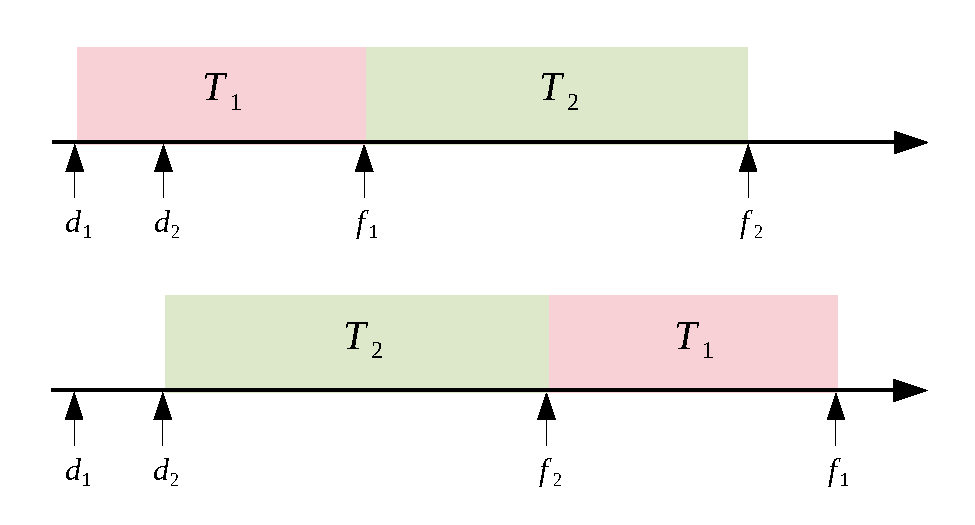
\includegraphics[scale=0.5]{Developpements/Ordonnancement online/ordo exemple.pdf}
\end{center}

Supposons que l'on veuille minimiser le temps de réponse maximal. On considère la stratégie \og Premier Arrivé Premier Servi \fg{} (PAPS) qui exécute chaque tâche dans leur ordre d'arrivé. 

\begin{theorem}
Étant donné $n$ tâches $T_i$, la stratégie PAPS minimise $\max_{1\leq i \leq n} R_i $.
\end{theorem}

\begin{proof}
Le but est d'appliquer une propriété d'échange. On considère un ordonnancement optimal $\mathcal{S}$, différent de la stratégie PAPS.  Ainsi, il existe deux tâches $T_i$ et $T_j$ telles que :
\begin{itemize}
\item $T_i$ est exécutée juste après $T_j$ (donc $f_j <f_i$) ;
\item alors que $T_i$ était disponible avant $T_j$ ($d_i <d_j$)
\end{itemize}
Regardons ainsi les temps de réponse dans $\mathcal{S}$. On a $R_i = f_i -d_i > f_j - d_j = R_j$. \newline

On construit alors un ordonnancement $\mathcal{S}'$ obtenu à partir de $\mathcal{S}$ en exécutant $T_i$ avant $T_j$. 


\begin{center}
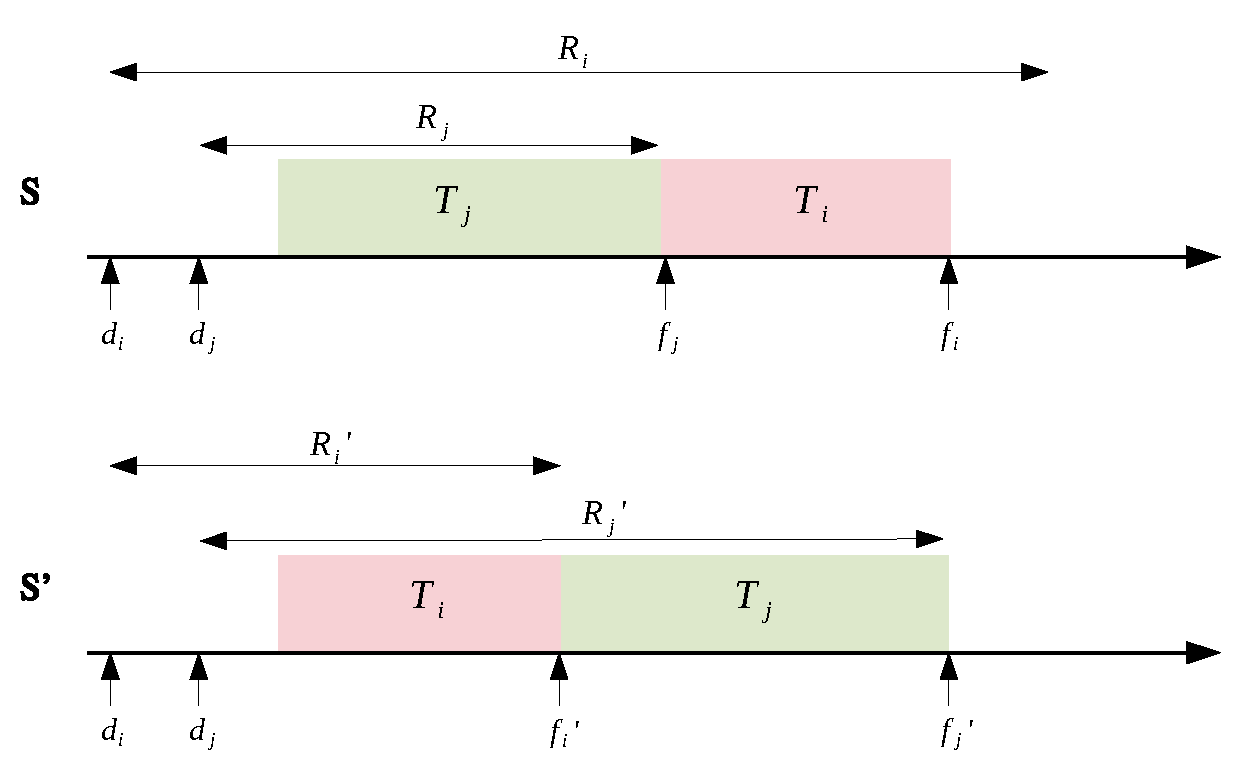
\includegraphics[scale=0.5]{Developpements/Ordonnancement online/ordo 2.pdf}
\end{center}

On remarque que les seuls temps de réponses changés sont ceux de $T_i$ et $T_j$. Or, on a 
$$
\left\lbrace \begin{array}{l}
R_i' = f_i'-d_i <f_i-d_i = R_i \\
R_j' = f_j' - d_j <f_i-d_j < f_i-d_i=R_i
\end{array}\right.
$$
Ainsi,  $\max(R_i',R_j') <R_i \leq \max(R_j,R_i)$. On en déduit alors que $S'$ est optimal. En appliquant successivement cette propriété d'échange, on peut alors se ramener à PAPS, montrant ainsi que cette stratégie est optimale.
\end{proof}

\begin{rem}
Si on veut minimiser cette fois la somme des temps de réponses $\sum_{i=1}^n R_i$, PAPS n'est plus optimale.
\end{rem}